\section{Knowledge-based factor}

The most used knowledge-based factors are passwords and PINs. 

\paragraph*{Advantages}
The advantages of passwords are: low cost, ease of deployment, and low technical barrier. 

\paragraph*{Disadvantages}
The primary drawbacks include the susceptibility of these secrets to:
\begin{itemize}
    \item Theft or snooping.
    \item Guessing by unauthorized individuals.
    \item Being cracked through various methods.
\end{itemize}

\paragraph*{Countermeasures}
Potential countermeasures include:
\begin{itemize}
    \item Regularly changing or expiring passwords to prevent prolonged exposure.
    \item Utilizing lengthy passwords with a diverse range of characters to enhance complexity.
    \item Ensuring that passwords are not directly associated with the user to deter predictable patterns.
\end{itemize}
To determine the most effective countermeasure, it's essential to anticipate the most probable attack in the given scenario.
Once identified, prioritize countermeasures that are feasible for users to follow and are likely to mitigate the identified threat effectively.

Countermeasures entail costs due to inherent human limitations. 
Unlike machines, humans struggle to effectively safeguard secrets, find it challenging to remember complex passwords, and cannot adopt an unlimited number of countermeasures.
\begin{table}[H]
    \centering
    \begin{tabular}{c|ccc}
                      & \textbf{Increase complexity} & \textbf{Change password} & \textbf{Not being user-related} \\ \hline
    \textit{Snooping} & $\tikzxmark$                 & $\tikzxmark$             & $\tikzxmark$          \\
    \textit{Cracking} & $\checkmark$                 & $\sim$                   & $\tikzxmark$          \\
    \textit{Guessing} & $\sim$                       & $\sim$                   & $\checkmark$    
    \end{tabular}
\end{table}

\subsection{User education and password complexity}
User education plays a critical role in addressing the human weakness, which often serves as the weakest link in security. 
This involves implementing policies to enforce strong passwords and regular password expiration or change. 
Additionally, employing password meters can help strike a balance between security and usability by guiding users in creating robust passwords.

When it comes to password complexity, it's essential to ensure that passwords contain a rich character set, including numbers, symbols, and both upper and lower-case letters. 
Moreover, passwords should be sufficiently long to resist brute-force attacks. 
Combining these elements enhances the strength of passwords and contributes to overall security.

\subsection{Secure password exchange}
At its core, authentication involves sharing a secret. To mitigate the risk of secrets being stolen, several strategies can be employed:
\begin{itemize}
    \item Implement mutual authentication whenever feasible.
    \item Utilize a challenge-response scheme, which involves exchanging random data to prevent replay attacks.
\end{itemize}
\begin{figure}[H]
    \centering
    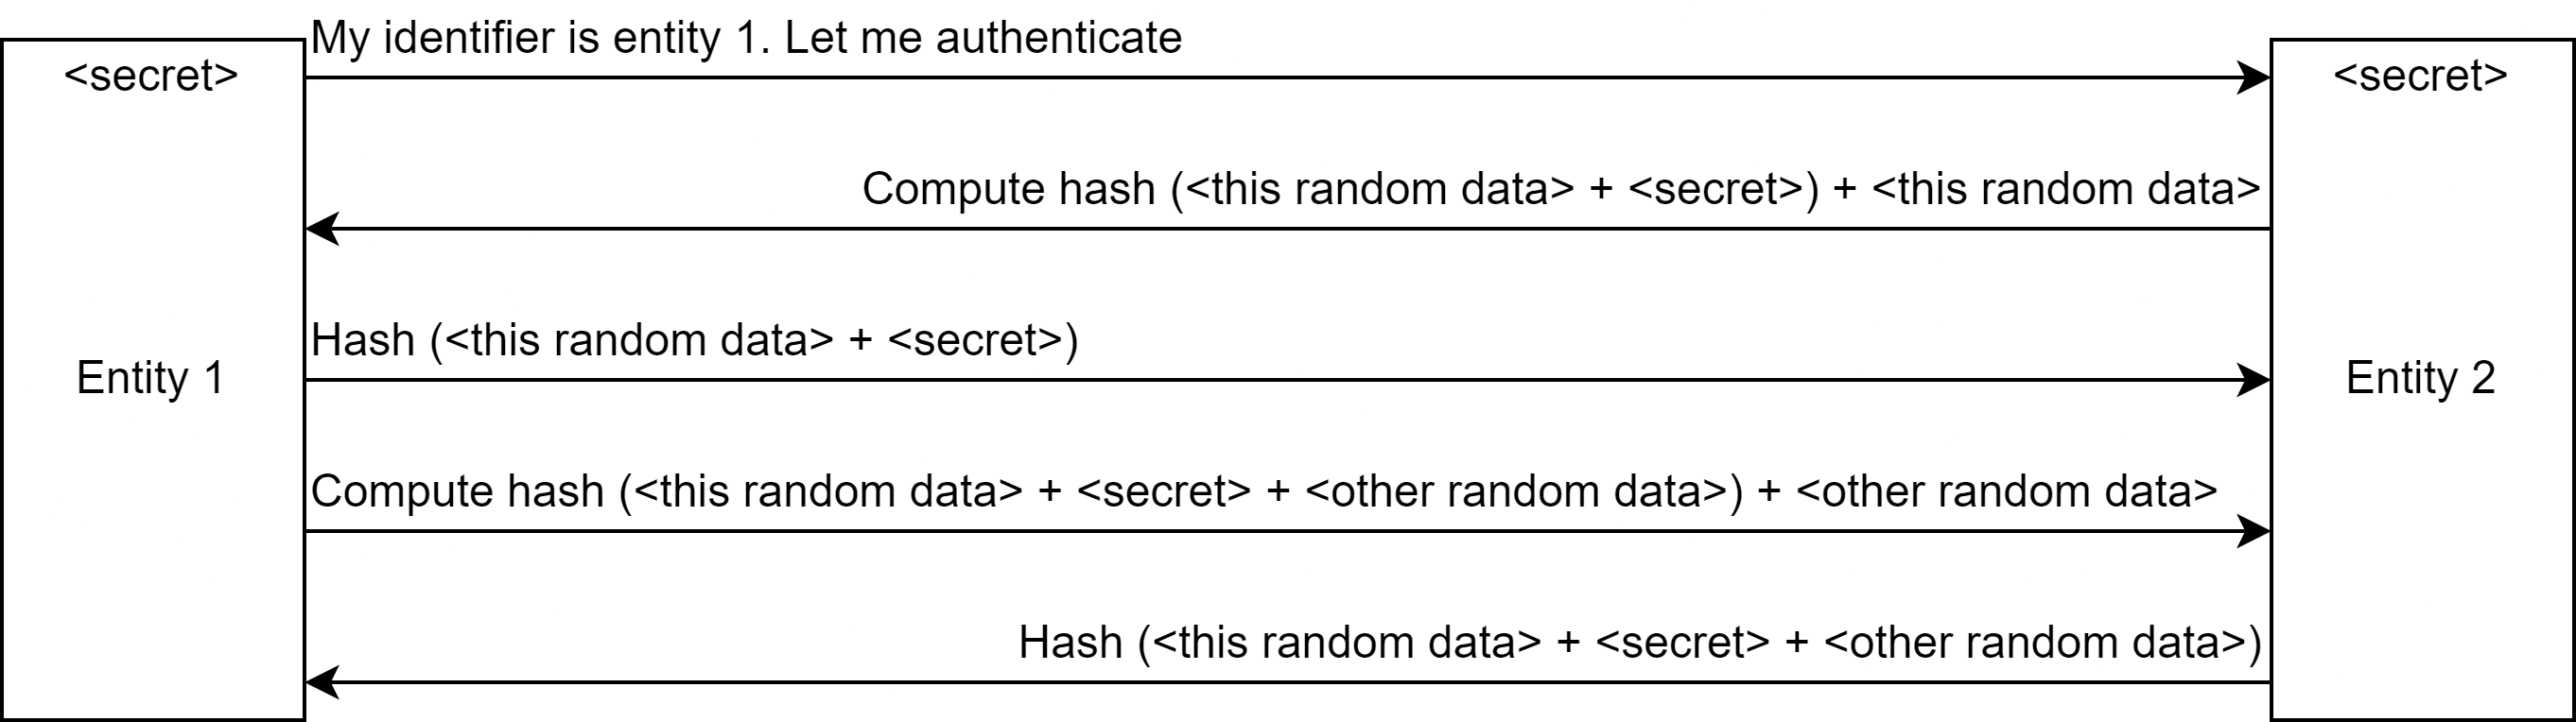
\includegraphics[width=0.75\linewidth]{images/auth2.png}
    \caption{Countermeasure costs}
\end{figure}

\subsection{Secure password storage}
To mitigate the risk of secrets being stolen from a file containing usernames and passwords stored by the operating system, several measures can be implemented:
\begin{itemize}
    \item Employ cryptographic protection: Ensure that passwords are never stored in clear text. 
        Instead, consider techniques such as hashing combined with salting to mitigate dictionary attacks.
    \item Implement access control policies: Limit privileges for reading and writing to the password file to authorized users only.
    \item Avoid disclosing secrets in password-recovery schemes: Ensure that password recovery mechanisms do not inadvertently reveal sensitive information.
    \item Address caching problems: Be mindful of information being stored in intermediate storage locations, as this can pose security risks. 
        Regularly review and manage cached data to minimize potential exposure.
\end{itemize}